\section{Processes}

Welcome to the final talk of this Practical Abhidhamma Course.\footnote{More details in Chapter 4 of “A Comprehensive Manual of Abhidhamma” (see Footnote 2 for link). \newline Also see \url{http://host.pariyatti.org/treasures/Process_of_Consciousness_and_Matter.pdf}} This talk will cover processes including the sensing process, thinking process and rebirth process.\footnote{The Abhidhammattha Sangaha also describes processes involved in attaining jhāna and attaining sainthood, but I have not included them as this is a “practical” course.} In other words, I will describe how there is seeing without a seer, how there is thinking without a thinker and how there is rebirth without a Self. From an Abhidhamma perspective, these processes involve a sequence of Mind Moments arising in a defined order.

For this talk, you should have Handouts 2, 9 10 in front of you. Handout 9 presents four ways to look at sensing and thinking: according to the Ball of Honey Sutta,\footnote{MN 18: \url{http://www.accesstoinsight.org/tipitaka/mn/mn.018.than.html}} according to “Objects,” according to the “Aggregates” and according to “Dependent Origination.” The top part of the handout, in grey, is related to sensing while the bottom part of the handout, in white, is related to thinking. Handout 10 shows the detailed sequence of Mind Moments as part of a seeing process, as part of a thinking process and as part of a rebirth process.

\subsection*{Importance of guarding the senses\footnote{For more information on guarding the senses, see Visuddhimagga I.50--59 (see footnote 2).}}

We will start by discussing the importance of guarding the senses.

A Buddhist scholar wrote,\footnote{Śāntideva (\url{http://en.wikipedia.org/wiki/Shantideva}) in his “Bodhisattvacaryāvatāra” (A Guide to the Bodhisattva’s Way of Life): \url{http://en.wikipedia.org/wiki/Bodhisattvacaryavatara}} “Where would I possibly find enough leather with which to cover the surface of the earth? Just the leather on the soles of my shoes is equivalent to covering the earth with it. Likewise, it is not possible for me to restrain the external course of things, but should I restrain my own mind, what would be the need to restrain all else?” In other words, it is not possible to see only nice things, hear only nice sounds, etc. The path of life is littered with sharp objects. Guarding the six senses does not change the nature of the world but it does offer protection.

\begin{figure}[h]
\centering
%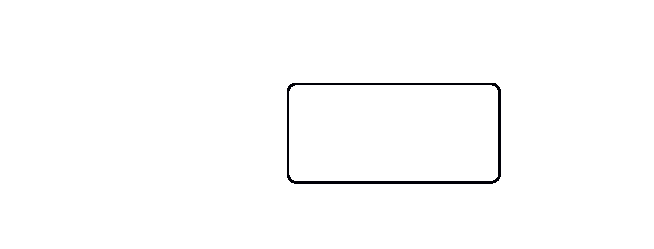
\includegraphics[width=0.7\linewidth]{./Diagrams/Feedback}
\input{./Diagrams/Feedback.pdf_tex}
\caption{The inputs to “The Mind” are objects arising arriving through the six sense doors. The outputs of “The Mind” are action, speech and thought. The activity of “The Mind” is influenced by accumulations, through natural decisive support condition. Thought is a mental phenomena and so a feedback loop can be created causing the “The Mind” to spin out of control in certain circumstances.}
\label{fig:Feedback}
\end{figure}

There is a story in the Commentary\footnote{\url{http://www.tipitaka.net/tipitaka/dhp/verseload.php?verse=282}; the specific instructions given by the seven-year-old Arahat to Poṭṭhila Thera are not included in the on-line translation, but are part of the Pāḷi original.} of a senior monk receiving instruction from a seven-year-old Arahat as follows, “To catch a lizard that has entered an ant-hill with six holes, one would cover five holes and keep watch at the sixth. Thus one should close the five senses, and watch the mind.”

The mind is the most difficult sense to guard because the mind loves to attach itself to things. Imagine that I ask you to hold up a cup. Initially, it is no problem but after a while the cup starts to feel heavy. While your hand is holding the cup, it cannot do anything else. If you were able to put the cup down for a short time, the muscles in your arm would be refreshed and you could easily pick up the cup again. The cup represents the things that obsess the mind. If the mind could let go of these things, even for a short time, the mind would be refreshed and would be available for other things.

The Buddha\footnote{MN 107: \url{http://www.accesstoinsight.org/tipitaka/mn/mn.107.horn.html}} had a gradual seven-step path to train monks, with each step building on the previous steps. The first step is morality, the second step is guarding the senses, the third step is moderation with food, the fourth is wakefulness, the fifth is \textbf{Mindfulness} of activities, the sixth is removing of the hindrances and the seventh step is attainment of the jhānas. In other words, guarding the senses is a very basic training for monks and for anybody looking to develop themselves spiritually. The Buddha warned, “On seeing a form with the eye, he does not grasp at its signs and features\footnote{“Signs and features” are the distinctive qualities of the object that can trigger latent defilements.} since if he left the eye-faculty unguarded, evil unwholesome states might invade him.”\footnote{Also found in MN 27: \url{http://www.accesstoinsight.org/tipitaka/mn/mn.027.than.html}}

The goal of spiritual development is to purify the mind. Purifying the mind doesn’t mean getting rid of impurities; it means guarding the senses so that impurities don’t get a chance to arise. When sense-objects are recognized, accepted, depersonalized and seen as they truly are,\footnote{\textit{\textbf{R}}ecognize, \textbf{\textit{A}}ccept, \textit{\textbf{D}}epersonalize, \textbf{\textit{I}}nvestigate, \textit{\textbf{C}}ontemplate \textbf{\textit{A}}\textit{nicca}/\textit{\textbf{C}}ontemplate \textbf{\textit{A}}\textit{nattā}, \textbf{\textit{L}}et go \\(the \textit{\textbf{RADICAL}} approach).} there are no conditions to support the arising of impurities and as a result, the mind is purified. This is how the senses are guarded.

The Buddha explained\footnote{AN 2.37: \url{http://obo.genaud.net/dhamma-vinaya/pts/an/02_twos/an02.031-040.wood.pts.htm}\\(see section [36]).} that the reason laypeople fight with other laypeople is \textbf{Attachment} to sense pleasures, fixation on sense pleasures, addiction to sense pleasures and obsession with sense pleasures. In other words, inability to guard the senses is the root cause of conflict, from marital squabbles to wars between countries. In the same Sutta, the Buddha explained that the reason one ascetic fights with other ascetics is \textbf{Attachment} to views, fixation on views, addiction to views and obsession with views.

Sensing happens automatically; it is the result of past kamma. Referring back to Handout 2, sensing is the input or trigger in the room analogy. The reaction to what is sensed creates new kamma. These are the four exits in the room analogy; three leading to the Danger Zone and one leading to the Faultless Zone. The reaction to the sense creates a new mental object. The new mental object is a new input or trigger of a thinking process causing a new reaction. The reaction of one thinking process becomes the object of the next thinking process and pretty soon, the mind is obsessing.

The Buddha\footnote{SN 36.6: \url{http://www.accesstoinsight.org/tipitaka/sn/sn36/sn36.006.nypo.html}} explained that both untrained worldlings (that’s us), and Arahats experience physical pain,\footnote{Buddha experienced physical pain: \url{http://www.tipitaka.net/tipitaka/dhp/verseload.php?verse=090}} but the difference is that untrained worldlings react to the physical pain with \textbf{Aversion} causing unpleasant mental \textbf{Feeling}, and this unpleasant mental \textbf{Feeling} causes more unpleasant mental \textbf{Feeling}. The mind of the untrained worldling obsesses over the unpleasant mental \textbf{Feeling} long after the physical painful \textbf{Feeling} has passed. The Buddha uses the simile of being struck by a dart once in the case of an Arahat, and being struck by a dart many times in the same spot in the case of untrained worldlings. In other words, sensing is the same for untrained worldlings and for Arahats, but thinking will be different.

If we allow obsessive thinking to dominate the mind, the experience of physical pain quickly becomes personalized as “my pain,” “I am in pain” or “it is painful to me.” Developing a habit of depersonalizing the experience of physical pain can be very beneficial. This can be done by practicing labeling the experience with cool detachment and \textbf{Mindfulness} as “pain has arisen,” observing the characteristics of the pain, or observing the Mind Moments that are aware of the physical pain.

Physical pain is an inescapable aspect of human existence. We all experience physical pain. For many people, physical pain arises near the time of death. Learning how to depersonalize the experience of physical pain now can be treated as a rehearsal to ensure a wholesome last Mind Moment.

\subsection*{The Ball of Honey Sutta (MN 18)}

\begin{figure}[H]
\begin{tabular*}{\textwidth}{C{\dimexpr0.5\textwidth-2\tabcolsep} | C{\dimexpr0.5\textwidth-2\tabcolsep}}
\toprule
\tableheader{Sensing\newline(generally result of past kamma)} & \tableheader{Thinking\newline(generally creates new kamma)} \\
\midrule
 Dependent on the eye and \textbf{Visible-forms}, eye-consciousness arises.\newline
 Dependent on the ear and \textbf{Sounds}, ear-consciousness arises.\newline
 Dependent on the nose and \textbf{Odours}, nose-consciousness arises.\newline
 Dependent on the tongue and \textbf{Tastes}, tongue-consciousness arises.\newline
 Dependent on the body and tactile objects, body-consciousness arises.\newline
 Dependent on the mind and dhammas, mind-consciousness arises.
 \newline\vspace{5mm}
 The meeting of the three is \textbf{Contact}.
 \newline\vspace{5mm}
 With \textbf{Contact} as a condition, there is \textbf{Feeling}.
 &
 What one feels, that one perceives.\newline
 What one perceives, that one thinks about.\newline
 What one thinks about, that one obsesses.\newline
 What one obsesses is the cause of perceptions and notions tinged by obsession that torment a person.
 \\
 
\bottomrule
\end{tabular*}
\caption{A portion of Handout 8, reformatted to focus on The Ball of Honey Sutta (MN 18).}
\end{figure}

Now let’s take a look at the Ball of Honey Sutta. In this Sutta, the Buddha is rudely asked by an arrogant layperson, “What do you teach?” The Buddha replied, “I teach in a way that one does not dispute with anybody,\footnote{In SN 22.94 (\url{http://suttacentral.net/en/sn22.94}), the Buddha says, “I do not dispute with the world; rather, it is the world that disputes with me. A proponent of the Dhamma does not dispute with anyone in the world.”} in a way that perceptions no longer awaken the latent defilements.” Later, some monks asked the Buddha to clarify this statement. The Buddha explained, “If there is nothing that is clung to, this is the end of latent defilements and this is the end of disputes.” The Buddha then left. 

\begin{figure}[h]
\centering
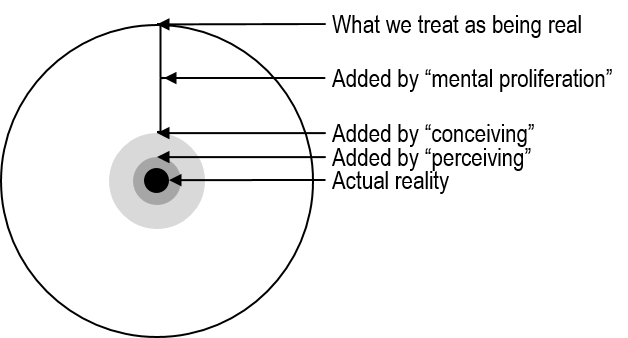
\includegraphics[width=0.55\linewidth]{./Diagrams/Reality}
\caption{Perceiving” identifies things. “Conceiving” imagines a relationship between the thing and a “Self.” “Mental proliferation” creates associations. All of these influence what we treat as being real.}
\label{fig:Reality}
\end{figure}

The monks were still confused, so they approached Mahākaccāna\footnote{Mahākaccāna: \url{http://en.wikipedia.org/wiki/Katyayana_(Buddhist)}} who was foremost in explaining in detail what the Buddha had explained in brief. Mahākaccāna explained, “Dependent on the eye and forms, eye-consciousness arises. The meeting of the three is \textbf{Contact}.\footnote{Eye-consciousness makes mental \textbf{Contact} (sense impression) with the \textbf{Visible-form} through the eye-base.} With \textbf{Contact} as a condition, there is \textbf{Feeling}. What one feels, that one perceives. What one perceives, that one thinks about. What one thinks about, that one obsesses.\footnote{The Pāḷi word that I have translated as “obsession” is “\textit{papañca}.” For a detailed analysis of this term see: \url{http://www.seeingthroughthenet.net/files/eng/books/other/concept_and_reality.pdf} Other translations of \textit{papañca} include “mental proliferation,” “mental construction,” “mental elaboration,” “the way in which the mind builds up or spins out of control because of craving, \textbf{Conceit} and \textbf{Wrong views}.”} What one obsesses is the cause of perceptions and notions tinged by obsession that torment a person. Dependent on the ear and \textbf{Sound}, ear-consciousness arises. The meeting of the three is \textbf{Contact}. With \textbf{Contact} as a condition, there is \textbf{Feeling}. What one feels, that one perceives. What one perceives, that one thinks about. What one thinks about, that one obsesses. What one obsesses is the cause of perceptions and notions tinged by obsession that torment a person.” and so on for each of the remaining four senses. In other words, when looking at Handout 9, Mahākaccāna repeated the same sequence six times, each time starting with a different sense. Mahākaccāna concluded by explaining that when there are no more obsessions, there are no more latent defilements and this is the end of disputes.\footnote{Obsession (\textit{papañca}) is also identified as the cause of disputes in DN 21 (\url{http://www.accesstoinsight.org/tipitaka/dn/dn.21.2x.than.html\#papanca}) as follows: obsession leads to thinking, which leads to desire, which leads to “dear-and-not-dear,” which leads to “\textbf{Envy} and \textbf{Stinginess},” which leads to disputes.} The Buddha later praises Mahākaccāna’s explanation and Ānanda says that in reflecting on this Sutta, a monk could find sweet satisfaction, just like a hungry man enjoying a Ball of Honey.\footnote{A large sweet cake or ball made of flour, ghee, molasses, honey, sugar, etc.}

The first part of the sequence, from “Dependent on...” through to “...there is \textbf{Feeling},” describes sensing. The language used is objective, describing an impersonal law of nature. The second part of the sequence, the part in white, describes thinking. The language used is subjective, describing one individual’s personal reaction. The transition from \textbf{Feeling} to perception is where the sequence moves from sensing to thinking and moves from impersonal to personal.

In an earlier talk, I mentioned a man with a latent fear of snakes. The man is walking down a dimly-lit path at night and there is a coil of rope ahead. His latent fear of snakes causes the man to misperceive the rope as a snake. This misperception together with his latent fear causes the man to think about snakes. This wrong thinking together with his latent fear convinces him that there is a snake and fear arises. You can see that misperception is the first step in the mind spinning out of control, of mental proliferation, of obsession.

\begin{figure} [H]

\setlength{\tabcolsep}{0pt}
\renewcommand{\arraystretch}{1.1}
%
\noindent\begin{tabular}{C{.18\textwidth}C{.15\textwidth}C{.2\textwidth}C{.2\textwidth}C{.27\textwidth}p{0\textwidth}}
\toprule
\tableheader{Individual} & \tableheader{Initial response} & \tableheader{Conceptual response} & \tableheader{Emotional response} & \tableheader{Reason} & \\
\midrule
Uninstructed worldling\newline(that's us \smiley) & Perceives & Conceives & Delights & Because he has not\newline fully understood & \\ [8mm]
Trainee: Sotāpanna/ Sakadāgāmī/ Anāgāmī & Directly knows & Open, therefore\newline let him not \newline conceive & Open, therefore\newline let him not\newline delight & In order that he might fully understand & \\ [8mm]
Arahat & Directly knows & Does not\newline conceive & Does not\newline delight & Fully understood; devoid of \textbf{Attachment}, \textbf{Aversion} \& \textbf{Delusion} & \\ [8mm]
Buddha & Directly knows & Does not\newline conceive & Does not\newline delight & Fully understood to the end; understands dependent origination & \\ [0mm]
\bottomrule

\end{tabular}

\caption[]{A summary of the Mūlapariyāya Sutta (MN 1) in tabular form. “Perceives” means . “Directly knows” means . “Conceives” means . Caption title\footnote{Temp} has a footnote!}

\end{figure}

\footnotetext{Temp example}

In another Sutta,\footnote{MN 1: \url{http://www.accesstoinsight.org/tipitaka/mn/mn.001.than.html} I am presenting an extremely simplified version of a very deep and difficult Sutta. For more details, please see \url{http://www.dhammatalks.net/Books11/Bhikkhu_Bodhi-Discourse_on_the_Root_of_Existence.pdf}} the Buddha explained that misperception is the root cause of wrong thinking in an untrained worldling. Ego-conceiving driven by craving, \textbf{Conceit} and Self-view distort how we think by twisting experience to match an egocentric view. The untrained worldling does not fully understand the object, so they take delight in it. The Arahat has eliminated Self-view, so he “directly knows” rather than misperceives. The Arahat fully understands the object, so he does not take delight in it.

According to Wikipedia,\footnote{\url{http://en.wikipedia.org/wiki/Rene_Descartes}} René Descartes has been dubbed the father of modern philosophy; his most famous statement is “I think, therefore I am.” Two thousand years before Descartes, the Buddha\footnote{Sn 4.14: \url{http://www.accesstoinsight.org/tipitaka/kn/snp/snp.4.14.than.html}} said that one should put a stop to the root of obsession which is the view, “I am the thinker.”

Imagine that I am walking down the street. \textbf{Visible-forms}, very small patches of colour, are repeatedly impinging on the eye. As a result, eye-consciousness is repeatedly arising, together with \textbf{Contact} and \textbf{Feeling}. The mind then starts the process of perception. The scene in front of me is glued together from all these small patches of colour. The mind starts recognizing shapes and then thinks about the whole image, “Oh that is a flower.” Next, the latent defilements of craving, \textbf{Conceit} and Self-view cause the mind to obsess, “I like flowers, my wife likes flowers, I should give my wife a flower. I imagine the smile on my wife’s face when I give her a flower.” You can see how my obsession causes me to lose touch with the reality of the present moment! And it all happened in a fraction of a second.

In that story, there were two levels of \textbf{Attachment}. The first level of \textbf{Attachment} was “craving for sense objects,” those very small patches of colour. At this point it is not a “flower” yet, it is simply a stimulation of the senses. To appreciate this “craving for sense objects,” imagine that you are sitting in a quiet room and there is a \textbf{Sound}. Does the mind not “run over to investigate the \textbf{Sound}?” Is the mind not attracted to anything new when something arises at the senses? Actually, this “craving for sense objects” is uprooted only by the Anāgāmī. This “craving for sense objects” is very subtle and does not create strong kamma. Much stronger kamma is created by the obsessions associated with thinking about the flower and the associations with the flower.

How would the mind of an Arahat function in this situation? Eye-consciousness together with \textbf{Contact} and \textbf{Feeling} would arise in the mind of the Arahat, just as they arise in my mind. However, the Arahat directly knows what arises as \textit{nāma} and \textit{rūpa}. The Arahat would use the name “flower,” but without any obsessing. As I mentioned in the first talk, the Buddha described names as “the world’s designations, the world’s expressions, the world’s ways of speaking, the world’s descriptions, with which the Buddha expresses himself but without grasping to them.”

As untrained worldlings, we spend most of our time caught up in obsessions and mental proliferations. Ever notice how these obsessions and mental proliferations always have a Self at the centre? These clouds of obsessions and mental proliferations conceal the true nature of experience. These obsessions and mental proliferations cause us to “personalize” the rose whereas the Arahat “depersonalizes” the rose.

Whenever we catch the mind indulging in obsession or mental proliferation, we should bring the mind back to the present moment using \textbf{Mindfulness}. Developing a habit of \textbf{Mindfulness} will reduce the ego, reduce the \textbf{Attachment} and reduce the \textbf{Aversion}. Life will constantly throw challenges at us, but a mind with less ego, less \textbf{Attachment} and less \textbf{Aversion} will make better decisions when facing these challenges.

\subsection*{Objects}

\begin{figure}[H]
\begin{tabular*}{\textwidth}{C{\dimexpr0.5\textwidth-2\tabcolsep} | C{\dimexpr0.5\textwidth-2\tabcolsep}}
\toprule
\tableheader{Sensing\newline(generally result of past kamma)} & \tableheader{Thinking\newline(generally creates new kamma)} \\
\midrule
\textbf{Visible-forms} / \textbf{Sounds} / \textbf{Odours} / \textbf{Tastes} / tactile objects / dhammas\newline
 (dhammas are ultimate realities; consciousness, mental factors and \textit{rūpa})
 &
 Names / ideas / concepts / judgements / obsessions / fantasies\newline
 (these objects are created by the mind)
 \\
 
\bottomrule
\end{tabular*}
\caption{A portion of Handout 8, reformatted to focus on Objects.}
\end{figure}

Now let’s look at the column labelled “Objects.” The objects listed in the grey portion are objects of sensing while the objects listed in the white portion are the objects of thinking. In the talk on \textit{rūpa}, we already discussed the first five objects in the grey portion (tactile objects are \textbf{Earth-element}, \textbf{Fire-element} and \textbf{Air-element}).

Dhammas\footnote{When capitalized, “Dhamma” usually refers to the Buddha’s teachings. In this Sutta, “dhamma” can be translated as “phenomenon” or Ultimate Reality. “Dhamma Theory” has been called the philosophical cornerstone of the Abhidhamma: \url{http://www.abhidhamma.com/Dhamma_Theory_clear.pdf}.} are objects of “mind-consciousness” and “mind.” “Dhammas” are the Ultimate Realities of consciousness, Mental Factors and \textit{rūpa}; \textit{Nibbāna} is not included in this list of “dhammas” because the experience of \textit{Nibbāna} does not fit into the definition of “sensing” or “thinking.”\footnote{Jhāna also does not fit the definition of “sensing” or “thinking.” The Abhidhammattha Sangaha details the jhāna experience and the experience of \textit{Nibbāna} as distinct processes from `sensing” and “thinking.”}

Consider the Ball of Honey Sutta verse, “Dependent on the mind and dhammas, mind-consciousness arises.” In this context, what do the terms “mind,” “dhammas” and “mind-consciousness” mean? Imagine that you are aware of an unpleasant mental \textbf{Feeling}. At that moment, the unpleasant mental \textbf{Feeling} is the object, it is a “dhamma.” This object, the unpleasant mental \textbf{Feeling}, is from a recent experience but it is distinct from the mind that is aware of the unpleasant mental \textbf{Feeling}. The aspect of the mind that is aware of the unpleasant mental \textbf{Feeling} is “mind-consciousness.” The aspect of the mind that provides a supporting base for “mind-consciousness” is called “mind;” “mind” is also the thing that connects the “mind-consciousness” (awareness) with all the other activities arising at that moment, including \textbf{Contact} and \textbf{Feeling}.\footnote{The 18 elements (\textit{dhātu}) are described in MN 115 (\url{http://www.yellowrobe.com/component/content/article/120-majjhima-nikaya/321-bahudhtuka-sutta-the-many-kinds-of-elements.html}) as “eye-element,” “visible-form-element,” “eye-consciousness-element,” “ear-element,” “sound-element,” “ear-consciousness-element,” ... “mind-element,” “dhamma-element (mind-object-element)” and “mind-consciousness element.” In the Abhidhamma, eye-consciousness-element is Mind Moment \textbf{13} and Mind Moment \textbf{20}, ear-consciousness-element is Mind Moment \textbf{14} and Mind Moment \textbf{21}, etc. “Mind-element” is Mind Moment \textbf{18}, Mind Moment \textbf{25} and Mind Moment \textbf{28}. The remaining 76 Mind Moments are “mind-consciousness-element.” “Mind-element” Mind Moments only arise through the sense-door whereas “mind-consciousness-element” Mind Moments can arise through the mind-door.}

Let’s consider the example of being aware of an unpleasant mental \textbf{Feeling} in a bit more detail because there is a practical lesson here. In the recent past, there was a Mind Moment accompanied by unpleasant \textbf{Feeling} and now there is a present Mind Moment that is aware of the recently-past unpleasant \textbf{Feeling}. The recently-past Mind Moment, the one with the unpleasant \textbf{Feeling}, was obviously unwholesome, \textbf{Aversion}-rooted, in the Danger Zone. However, the present Mind Moment, the one that is taking the recently-past \textbf{Feeling} as its object, is wholesome; to quote the \textit{Satipaṭṭhāna} Sutta, “when there is unpleasant \textbf{Feeling}, he knows that there is unpleasant \textbf{Feeling}.”

We know that once the mind experiences an unpleasant mental \textbf{Feeling}, the mind often spins out of control. The mind keeps returning to the same undesirable object and the level of \textbf{Aversion} keeps growing. \textbf{Aversion} feeds more \textbf{Aversion} until the mind is consumed and obsessed by \textbf{Aversion}.

When a wholesome moment with \textbf{Mindfulness} arises, this temporarily interrupts the negative spiral. At least for a moment, the mind’s object is not the thing that triggered the unpleasant Mind Moment, the mind’s object is inward-looking, focusing on the recently-past Mind Moment. The flow of negativity has a lot of momentum, so one moment with \textbf{Mindfulness} is not going to stop it. If there are many moments with \textbf{Mindfulness}, the descent can be slowed.

In other words, repeated \textbf{Mindfulness} stops \textbf{Aversion}-based Mind Moments such as anger, fear, depression and \textbf{Remorse} from growing. Similarly, repeated \textbf{Mindfulness} stops \textbf{Attachment}-based Mind Moments such as lust, greed and \textbf{Conceit} from growing. Training the mind to apply repeated \textbf{Mindfulness} will have ongoing beneficial effects during daily life. \textit{Vipassanā} meditation trains the mind to apply repeated \textbf{Mindfulness}.

As we transition from sensing to thinking, the nature of the object changes. The white portion of the “Objects” column lists “names, ideas, concepts, judgements, obsessions and fantasies” as objects of thinking. These objects are created by the mind and fall under the general category of “concepts” (things distinct from the Ultimate Realities).

Concepts themselves are not a problem (an Arahat also uses concepts); it is how concepts are handled that creates problems. It is almost impossible to communicate, verbally or in writing, without using names and ideas. I consider names and ideas to be “harmless” concepts in the sense that they are not dangerous. However, when defilements or emotions mix with these “harmless” concepts, they quickly become dangerous as suggested by the terms, “judgements, obsessions and fantasies.” As the mode of thinking described in the Ball of Honey Sutta progresses from “perceiving” to “thinking about” to “obsessing,” the nature of the object moves from “harmless” to “dangerous.” An Arahat uses names and ideas, but has no judgements, obsessions or fantasies.

I have seen a tee shirt from a meditation centre that reads, “Lost in thought? Come back to your senses.” If we find ourselves judging, obsessing and fantasizing, we should leave the Danger Zone and note what is happening at the present moment. This reminds me of a joke: a meditation master says to the yogi, “I have never met anyone so thoughtless in my life, keep up the good work!”

A great time to come back to your senses is just before going to sleep. Use the time before you go to sleep to be aware of the sensations of the body. Scan the body and note any internal sensations\footnote{If the scanning of internal sensations detects tension, you can either simply note the tension or try to relax the tension. Simply noting the tension is a \textbf{Mindfulness} exercise. Trying to relax the tension is a relaxation exercise.}. Experience your head resting against the pillow, experience your back touching the mattress and experience the cover on your chest. If the mind starts reviewing the past or planning the future or getting lost in a fantasy, bring the mind back to experiencing bodily sensations. Replacing ego-centric thoughts of reviewing, planning or fantasizing with \textbf{Mindfulness} for a few minutes a day may not seem like a big deal, but every drop helps to fill the bucket and reinforces a habit of \textbf{Mindfulness}.

\subsection*{Aggregates\footnote{For an in-depth analysis of the aggregates, see \url{http://www.ahandfulofleaves.org/documents/Identity and Experience_Hamilton_1996.pdf} and \url{http://www.ahandfulofleaves.org/documents/The Five Aggregates_Understanding Theravada Psychology and Soteriology_Boisvert.pdf}}}

\begin{figure}[H]
\begin{tabular*}{\textwidth}{C{\dimexpr0.5\textwidth-2\tabcolsep} | C{\dimexpr0.5\textwidth-2\tabcolsep}}
\toprule
\tableheader{Sensing\newline(generally result of past kamma)} & \tableheader{Thinking\newline(generally creates new kamma)} \\
\midrule
Material aggregate:\newline
 Non-mental phenomena\newline\vspace{5mm}
 
 Consciousness aggregate:\newline
 Eye-consciousness, ear-consciousness, nose-consciousness, tongue-consciousness, body-consciousness and mind-consciousness\newline\vspace{5mm}
 
 \textbf{Feeling} aggregate:\newline
 \textbf{Feeling} born of \textbf{Contact} through the eye, ear, nose, tongue, body and mind
 &
 \textbf{Perception} aggregate:\newline
 \textbf{Perception} of \textbf{Visible-forms}, \textbf{Sounds}, \textbf{Odours}, \textbf{Tastes}, tactile objects and mental phenomena
 \newline\vspace{5mm}
 Volitional formations aggregate:\newline
 \textbf{Volition} regarding \textbf{Visible-forms}, \textbf{Sounds}, \textbf{Odours}, \textbf{Tastes}, tactile objects and mental phenomena
 \\
 
\bottomrule
\end{tabular*}
\caption{A portion of Handout 8, reformatted to focus on Aggregates.}
\end{figure}

Let’s move to the column titled, “Aggregates.” The five aggregates are the Buddha’s way of describing what is conventionally considered to be Self. This teaching is core to Buddhism. In the talk on Mental Factors, I suggested that it is useful to look at Mental Factors as both nouns and verbs. Similarly, one can look at aggregates as both nouns (the “components” of a being) and as verbs (the “activities” of a being).

After his enlightenment, the Buddha reunited with the five ascetics who had been his companions and gave the fundamentals of his teaching in his first sermon.\footnote{SN 56.11: \url{http://www.accesstoinsight.org/tipitaka/sn/sn56/sn56.011.harv.html}} After the sermon, only one of the five ascetics\footnote{Añña-Koṇḍañña, the other four ascetics were Bhaddiya, Vappa, Mahānāma and Assaji.} was able to attain the first degree of sainthood. It was not until the second sermon,\footnote{SN 22.59: \url{http://www.accesstoinsight.org/tipitaka/sn/sn22/sn22.059.mend.html}} when the Buddha talked about the aggregates and non-self, were the ascetics able to become Arahats.

I mentioned that concepts themselves are not a problem, it is how concepts are handled that creates problems. Similarly, the five aggregates are not a problem (an Arahat also has five aggregates), it is the “five clinging aggregates” that the Buddha equated with suffering. Clinging to aggregates is Self-view and Self-view is a cause of suffering.

If you look at the presentation of the Ball of Honey Sutta, the sensing section, the three grey boxes, actually arise simultaneously. The thinking section, the white box, has a sequential progression from “harmless” to “dangerous.” The five aggregates always arise simultaneously, but in Handout 9 they have been grouped according to the relevance of the role that they play in the presentation of the Ball of Honey Sutta.\footnote{In the Suttas, the aggregates are always presented in the order of \textit{rūpa}, \textbf{Feeling}, \textbf{Perception}, volitional formations and then consciousness. This probably represents a progression from the coarsest, most easily observed (\textit{rūpa}), to the most subtle (consciousness).}

The five aggregates can be described from an Abhidhamma perspective as follows. The \textit{rūpa} aggregate and the consciousness aggregate correspond to the \textit{rūpa} and consciousness Ultimate Realities from the Abhidhamma. The \textbf{Feeling} aggregate and the perception aggregate correspond to two Mental Factors from the Abhidhamma and the volitional formations aggregate corresponds to the remaining fifty Mental Factors from the Abhidhamma, with \textbf{Volition} being the most important.

That the five aggregates can be described from an Abhidhamma perspective is not surprising. What you may find surprising is that in the Suttas, four of the five aggregates (all except \textit{rūpa}) are described based on sensing and thinking. The Buddha\footnote{SN 22.56: \url{http://www.accesstoinsight.org/tipitaka/sn/sn22/sn22.056.than.html}} described the aggregate of consciousness as having six classes; eye-consciousness, ear-consciousness, etc. He described the aggregate of \textbf{Feeling} as having six classes; \textbf{Feeling} born of \textbf{Contact} through the eye, \textbf{Feeling} born of \textbf{Contact} through the ear, etc. He described the perception aggregate as having six classes; perception of \textbf{Visible-form}, perception of \textbf{Sound}, etc. He described aggregate of volitional formations as having six classes; volitional formations regarding \textbf{Visible-form}, volitional formations regarding \textbf{Sound}, etc.

The Suttas describe the \textit{rūpa} aggregate in a standard way as, “The four great elements and the \textit{rūpas} derived from the four great elements,” but this can also be linked to sensing because as the Ball of Honey Sutta mentions, the conditions leading to the arising of consciousness are the occurrence of the internal sense organ \textit{rūpa} with an external sense object \textit{rūpa}.\footnote{MN 28: \url{http://www.accesstoinsight.org/tipitaka/mn/mn.028.than.html} also mentions a third required factor of “\textit{tajjo samannāhāro}” (translated as “a corresponding engagement”). The Commentary identifies this as the Mental Factor of \textbf{Attention} (\textit{manasikāra}) in Mind Moment \textbf{28}. In other words, even when a \textbf{visible-form} come into the range of the eye, if \textbf{Attention} is not engaged by the \textbf{Visible-form} because one is occupied with something else, then there is no manifestation of the “corresponding type of consciousness” (i.e. eye-consciousness).}

Though \textbf{Perception} and volitional formations arise together, I have shown a progression from \textbf{Perception}, which focuses more on the “harmless” aspects of the object, to volitional formations which play a more important role with the “dangerous” aspects of this object. This is because “dangerous” emotions are associated with the volitional formations aggregate rather than with the “harmless” objects of the \textbf{Perception} aggregate.

The objects of \textbf{Perception} and volitional formations include “mental phenomena.” This term “mental phenomena” would include both the dhammas (Ultimate Realities) and the types of objects listed under thinking (names, ideas, concepts, etc.).

\subsection*{Dependent Origination}

\begin{figure}[H]
\setlength{\tabcolsep}{0pt}
\renewcommand{\arraystretch}{0.9}
\begin{center}
\noindent\begin{tabular}{C{.1\textwidth}C{0.4\textwidth}}
\toprule

\multirow{3}{.1\textwidth}{Past causes} & Ignorance (\textit{Avijjā}) \\
& ↓ \\
& Kammic formations (\textit{Saṅkhāra}) \\
\cmidrule{1-1}
& ↓ \\
\cmidrule{1-1}
\multirow{9}{.1\textwidth}{Present effects} & Consciousness (\textit{Viññāṇa})\\
& ↓ \\
& Mind \& matter (\textit{Nāma-rūpa})\\
& ↓ \\
& Six sense bases (\textit{Saḷāyatana})\\
& ↓ \\
& Contact (Phassa)\\
& ↓ \\
& Feeling (Vedanā)\\
\cmidrule{1-1}
& ↓ \\
\cmidrule{1-1}
\multirow{5}{.1\textwidth}{Present causes} & Craving (\textit{Taṇhā})\\
& ↓ \\
& Clinging (\textit{Upādāna})\\
& ↓ \\
& Existence (\textit{Bhava})\\
\cmidrule{1-1}
& ↓ \\
\cmidrule{1-1}
\multirow{3}{.1\textwidth}{Future effects} & Birth (\textit{Jāti})\\
& ↓ \\
& Decay \& death (\textit{Jarā-maraṇa})\\

\bottomrule

\end{tabular}
\end{center}

\caption{Links in dependent origination}

\end{figure}





\begin{figure}[H]
\begin{tabular*}{\textwidth}{C{\dimexpr0.5\textwidth-2\tabcolsep} | C{\dimexpr0.5\textwidth-2\tabcolsep}}
\toprule
\tableheader{Sensing\newline(generally result of past kamma)} & \tableheader{Thinking\newline(generally creates new kamma)} \\
\midrule
Six sense bases:\newline
 Eye-base / ear-base / nose-base /\newline tongue-base / body-base / mind-base\newline\vspace{5mm}
 \textbf{Contact}:\newline
 Mental Factor of \textbf{Contact} arising in Mind Moments that are the result of past kamma\newline\vspace{5mm}
 \textbf{Feeling}:\newline
 Mental Factor of \textbf{Feeling} arising in the same Mind Moments as \textbf{Contact}
 &
 Craving:\newline
 Craving for sense objects\newline (\textbf{Visible-forms}, \textbf{Sounds}, \textbf{Odours}, \textbf{Tastes},\newline tactile objects and mental phenomena)
 \newline\vspace{5mm}
 Clinging:\newline
 Sense-desire clinging, false-view clinging, rite-and-ritual clinging, self-clinging
 \\
 
\bottomrule
\end{tabular*}
\caption{A portion of Handout 8, reformatted to focus on Dependent Origination.}
\end{figure}

As shown in Handout 9, sensing and thinking are also at the core of dependent origination (\textit{paṭiccasamuppāda}). In fact, there is another Sutta\footnote{SN 12.44: \url{http://www.accesstoinsight.org/tipitaka/sn/sn12/sn12.044.than.html}} that starts in the same way as the Ball of Honey Sutta, “Dependent on the eye and forms, eye consciousness arises. The meeting of the three is \textbf{Contact}. With \textbf{Contact} as a condition, there is \textbf{Feeling}.” and then jumps to the links of dependent origination, “from \textbf{Feeling} comes craving, from craving comes clinging, etc.”

Before discussing the six sense bases, let me give you a quick summary of the traditional links in dependent origination\footnote{SN 12.2: \url{http://www.accesstoinsight.org/tipitaka/sn/sn12/sn12.002.than.html}} that lead up to the six sense bases. Dependent origination describes the natural set of conditions that keep us bound to \textit{saṃsāra}. You might say that dependent origination is the “macro-view,” while the Ball of Honey Sutta is the “day-to-day-view” and the Abhidhamma is the “microscopic-view.”

The traditional interpretation of dependent origination is that it spans three lifetimes;\footnote{There is a modern reinterpretation of dependent origination in which all links arise in a single moment.} the past lifetime, the present lifetime and a future lifetime. The past lifetime starts\footnote{Though ignorance is the first link in dependent origination, it is not a “first cause;” ignorance also arises due to conditions. According to the Commentary, “unwise \textbf{Attention}” is the proximate cause of ignorance.} with ignorance\footnote{Mental Factor of \textbf{Delusion} in Mind Moment \textbf{1}--\textbf{12}.} which is a condition\footnote{For the conditions involved, see Visuddhimagga XVII.102--104 (see footnote 2).} for kammic formations.\footnote{Mental factor of \textbf{Volition} in kamma-creating Mind Moments that can condition rebirth (all Mind Moments in the top row of Handout 2, except the supramundane path; Mind Moments \textbf{82}--\textbf{85}).} The kammic formations from the previous life are a condition\footnote{Kamma and natural decisive support condition rebirth; Visuddhimagga XVII.177--181 (see footnote 2).} for rebirth-linking consciousness\footnote{The Life-continuum Mind Moment; for humans, Mind Moment \textbf{27}, \textbf{39}--\textbf{46}.} of the present life to arise.

Within this lifetime, rebirth-linking consciousness supported by kammic formations from the past life are a condition\footnote{SN 12.67 (\url{http://www.accesstoinsight.org/tipitaka/sn/sn12/sn12.067.than.html}) explains that \textit{nāmarūpa} arises with consciousness as a condition and also consciousness arises with \textit{nāmarūpa} as a condition, just like two sticks mutually supporting each other.} for the arising of the mind and body.\footnote{Visuddhimagga XVII.201 (see footnote 2) defines consciousness, \textit{nāmarūpa} and their link.} Conditioned by mind and body, the six sense bases arise.\footnote{Visuddhimagga XVII.207--217 (see footnote 2) defines \textit{nāmarūpa}, six sense bases and their link.} This is the portion of dependent origination that leads up to what is shown on Handout 9.

The six sense bases\footnote{Visuddhimagga XVII.227 (see footnote 2) defines six sense bases, \textbf{Contact} and their link.} are eye-base, ear-base, nose-base, tongue-base, body-base and mind-base. According to the Abhidhamma, the first five of these are the five sense organ \textit{rūpas}: \textbf{Eye-sensitivity}, \textbf{Ear-sensitivity}, etc. and the mind-base is \textit{citta}, consciousness.

\textbf{Contact} is the Mental Factor of \textbf{Contact} arising in Mind Moments that are the result of past kamma. So eye-\textbf{Contact} is the Mental Factor in Mind Moments \textbf{13} and \textbf{20}, ear-\textbf{Contact} is the Mental Factor in Mind Moments \textbf{14} and \textbf{21}, etc. and mind-\textbf{Contact} is the Mental Factor of \textbf{Contact} arising in Mind Moments \textbf{18}, \textbf{19}, \textbf{25}--\textbf{27}, \textbf{39}--\textbf{46}, \textbf{60}--\textbf{64} and \textbf{74}--\textbf{77}. In other words, mind-\textbf{Contact} is the Mental Factor of \textbf{Contact} arising in all the remaining “Result of Past Kamma” Mind Moments except the Supramundane Fruit.

Feeling\footnote{Visuddhimagga XVII.231 (see footnote 2) defines \textbf{Contact}, \textbf{Feeling} and their link.} is the Mental Factor of \textbf{Feeling} arising in the same Mind Moments in which the Mental Factor of \textbf{Contact} arises. Earlier, I mentioned that consciousness and all of the associated Mental Factors arise simultaneously in a Mind Moment. In other words, \textbf{Contact} and \textbf{Feeling} arise at the same time in the same Mind Moment; they are not sequential.

The Abhidhamma defines 24 conditions that relate one Ultimate Reality to another and the Commentaries define additional sub-categories of conditions.\footnote{More details in Chapter 8 of “A Comprehensive Manual of Abhidhamma” and “The Conditionality of Life” (see Footnote 2 for links).} In the previous talk, I described kamma condition and natural decisive support condition. I consider these two conditions to be the “interesting” ones because an understanding of kamma and natural decisive support can be directly applied to one’s daily \color{blue} practice\color{black}. I consider the remaining conditions to be “boring” because they are very technical.

A few of the “boring” conditions link \textbf{Contact} to the six sense bases and another set of “boring” conditions link \textbf{Feeling} to \textbf{Contact}. These are the conditions that are part of sensing; the objective, impersonal laws of nature. The “interesting” conditions, specifically natural decisive support, play a role when we move into thinking; the subjective, personal, individual’s reaction to what is sensed.

As shown in Handout 9, craving\footnote{Visuddhimagga XVII.237 (see footnote 2) defines \textbf{Feeling}, craving and their link.} is craving for sense objects, including craving for mental phenomena. From an Abhidhamma perspective, craving is the Mental Factor of \textbf{Attachment} arising in Mind Moments \textbf{1}--\textbf{8}.

Clinging\footnote{Visuddhimagga XVII.248 (see footnote 2) defines craving, clinging and their link.} includes sense-desire clinging, false-view clinging, rite-and-ritual clinging and Self-clinging. From an Abhidhamma perspective, clinging is the Mental Factor of \textbf{Attachment} to \textbf{Wrong view} arising in Mind Moments \textbf{1}, \textbf{2}, \textbf{5} and \textbf{6}.

Sense-desire clinging arises at the same time as craving as they both take the sense-object as their object. The other three kinds of clinging (false-view clinging, rite-and-ritual clinging and Self-clinging) can arise together with craving or they can arise later. To appreciate how clinging can arise later, consider the story of the man with a latent fear of snakes. The sense object was the trigger, but the latent fear used this trigger to create a distorted perception, then a distorted thought and then a distorted view.

According to the Abhidhamma, there is only one condition that links craving back to \textbf{Feeling}; natural decisive support condition. To put it bluntly, it is only our bad habits that keep us bound to \textit{saṃsāra}. When clinging arises together with craving in the same Mind Moment, a set of “boring” conditions are involved. When clinging arises later than craving, then natural decisive support plays a role. In other words, distorted perception, distorted thought and distorted views arise because of bad habits.

You will see that in Handout 9 I used a sloped line between perception aggregate and volitional formations aggregate. I also used a sloped line between craving and clinging. Volitional formations build upon perception and clinging builds upon craving, but there is no one-to-one correspondence between perception and craving and no one-to-one correspondence between volitional formations and clinging.

Before leaving the topic of dependent origination, let me complete the sequence that arises after clinging. Conditioned by clinging, becoming arises.\footnote{Visuddhimagga XVII.269 (see footnote 2) describes clinging, becoming and their link.} In this context, “becoming” means the creating of new kamma. Conditioned by this new kamma, birth in the next existence arises,\footnote{Rebirth is conditioned by kamma and natural decisive support.} and with rebirth in the next existence arises ageing, sorrow, pain and death.\footnote{Visuddhimagga XVII.270 (see footnote 2) describes the factors and the links involved.} Reminds me of a joke: the Buddhist coroner was fired because he kept marking the cause of death as “birth.” 

\subsection*{Handout 10}

Let’s now move to the final handout, Handout 10, titled “Processes.” As you can see, it includes an example Sensing Process, an example Thinking Process and an example Death and Rebirth Process. The Abhidhammattha Sangaha and later Commentaries describe many variations of these processes, but in this Practical Abhidhamma course we will focus on a single example for each.

In the first talk, I mentioned that the Abhidhamma provides a simple model of how the mind works. I used an example of the water cycle to show how a simple model can help us to understand something very complex as being a natural phenomena. Handout 10 shows very simple models to help us to understand that the complicated processes of sensing, thinking, death and rebirth are actually natural phenomena.

Before going into the detailed models shown in Handout 10, here is a high-level analogy. Consider a burning candle. The wax of the candle is the body and the wick is the sense organ. The oxygen in the atmosphere is the sense object, and the candle flame that arises dependent on the wick and the oxygen is the Mind Moment that arises dependent on the sense organ and the sense object. The flame that exists now is not the same as the flame that existed a minute ago, but the two are linked because the earlier flame is a condition for the arising of the later flame. The Mind Moment that exists now is not the same as the Mind Moment that existed a minute ago, the two are linked because the earlier Mind Moment is a condition for the arising of the later Mind Moment. If the flame from one candle is used to light the wick of another candle, the previous flame is a condition for the arising of the subsequent flame, even though the subsequent flame is part of a new candle; new wax and new wick. At the moment of rebirth, the Mind Moment from a past being “ignites” the Mind Moment in a new being; the new being has a new body and new sense organs.

In each example shown in Handout 10, the mind is represented by a series of circles arising one after another in sequence. Each circle represents a single Mind Moment, one of the 89 Mind Moments shown in Handout 2.

This model shows that the sequence of Mind Moments is continuous, never stopping.\footnote{There are two cases where the flow of Mind Moments is suspended for a time; beings in Realm \textit{22} (Gods without Consciousness) and during a meditative state called “Attainment of Cessation Process” (\textit{nirodha-samāpatti vīthi}), which is only available to an Anāgāmī or an Arahat.} Even during the death and rebirth, the flow of Mind Moments continues, though the \textit{rūpa} supporting the mind changes at the moment of rebirth.

The model also shows that there is only one Mind Moment at a time.\footnote{I used a circle to indicate that each Mind Moment has three sub-moments; arising (\textit{uppāda}), presence (\textit{ṭhiti}) and dissolution (\textit{bhanga}). This distinction becomes important when discussing \textit{rūpa}.} The falling away of one Mind Moment is a necessary condition for the arising of the subsequent Mind Moment.\footnote{In the \textit{Paṭṭhāna}, this is called “Proximity condition” (\textit{anantara-paccaya}) and “Contiguity condition” (\textit{samanantara-paccaya}). More details in Chapter 5 of “The Conditionality of Life” (see Footnote 2).} It may seem that sensing and thinking arise at the same time or that seeing and hearing happen simultaneously, but the Abhidhamma tells us that these processes arise in extremely quick succession; sequentially, not in parallel. According to the Commentary, billions of Mind Moments arise and fall away in the duration of a lightning flash or in the blink of an eye.

Finally, the models show that Mind Moments arise in a specific sequence, according to a “natural, fixed law of the sequence of Mind Moments.”\footnote{The Commentary refers to this “natural, fixed law of the sequence of Mind Moments” as \textit{citta-niyāma}. Other natural, fixed
laws defined in the Commentary cover temperature, seasons and physical events (\textit{utu-niyāma}), plant life
(\textit{bīja-niyāma}), the workings of kamma (\textit{kamma-niyāma}) and certain events connected with the
Dhamma (\textit{dhamma-niyāma}) such as events occurring in the lives of Buddhas.} In other words, the Mind Moments do not appear in a random order.

\subsection*{Sensing Process}

\begin{figure}[h]
\centering
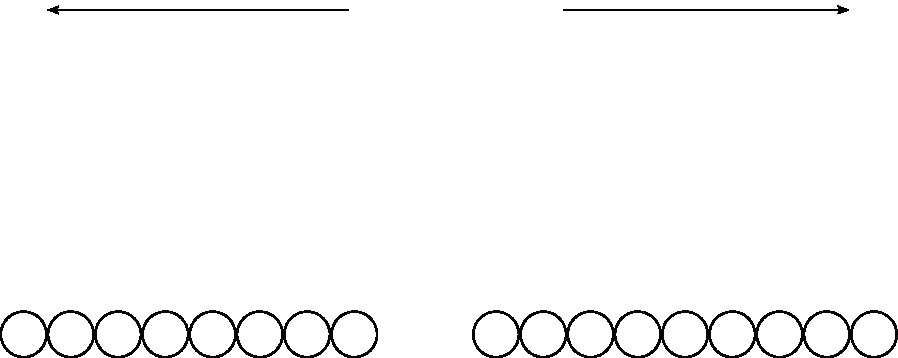
\includegraphics[width=1\linewidth]{./Diagrams/Process}
\caption{An example of a Sensing Process; an Eye-door Process that shows how seeing happens without a seer.}
\label{fig:Process}
\end{figure}

The example Sensing Process shown in Handout 10 is an Eye-door Process that shows how seeing happens without a seer.

The Commentary gives a simile of a mango tree to illustrate the Sensing Process. A man sleeps beneath a mango tree (Stream of Life-continuum). A wind strikes the tree (Past Life-continuum). The branches sway with the wind (Vibrating Life-continuum). A mango falls beside the sleeping man (Arresting Life-continuum). The man awakes (Five-sense-door Adverting). The man opens his eyes (Eye-consciousness). The man picks up the mango (Receiving). The man presses and smells the mango (Investigating). The man understands that this is a mango fruit, ripe and ready to eat (Determining). The man eats the mango (Reaction). The man notes the after-taste; his saliva still retains the mango taste (Registration). The man falls back to sleep (Stream of Life-continuum).

This mango tree simile gives a general overview of the Sensing Process. Now let’s look at each Mind Moment in the sequence in detail.

\subsubsection*{Stream of Life-continuum}

Before the \textbf{Visible-form} exists, there are a large number of Life-continuum Mind Moments. All Life-continuum Mind Moments are identical, but some are given names according to what is occurring at that time. For example, the first Mind Moment in an existence is called “Rebirth-linking Mind Moment” and the last Mind Moment in an existence is called “Death Mind Moment,” but these are both Life-continuum Mind Moments. Life-continuum Mind Moments arise between processes and during dreamless sleep.

The object of all Life-continuum Mind Moments is taken from the prior existence and can be “kamma,” “sign of kamma” or “sign of destiny.” This object is “inherited” from the Death Process of the prior existence. 

A “kamma object” may be something like a memory of doing dāna or a memory of studying the Dhamma during the prior existence. A “sign of kamma object” may be something like a stethoscope (for a doctor) or a Buddha statue. A “sign of kamma object” represents wholesome or unwholesome actions done during the prior existence. 

There is a story in the Commentary\footnote{\url{http://www.tipitaka.net/tipitaka/dhp/verseload.php?verse=015}} about a cruel butcher. Before he died, he behaved like a terrified pig in pain. The butcher was experiencing the “past kamma” or the “sign of kamma” that would condition his rebirth. Another story in the Commentary\footnote{\url{http://www.tipitaka.net/tipitaka/dhp/verseload.php?verse=016}} speaks of a virtuous, generous lay disciple. On his death bed, he saw heavenly chariots waiting to transport him to a \textit{Deva} realm. This is an example of a “sign of destiny.”

\subsubsection*{Past/Vibrating/Arresting Life-continuum}

The first three Mind Moments of the Sensing Process are Life-continuum Mind Moments with names describing what is occurring at this time; Past Life-continuum, Vibrating Life-continuum and Arresting Life-continuum.

During “Past Life-continuum” the flow of Life-continuum is unperturbed by the \textbf{Visible-form} that has arisen. The Mind Moment is fixed firmly on the past object, an object from the previous existence. In the mango tree simile, this is when the wind strikes the tree while the man is sleeping.

During “Vibrating Life-continuum” the flow of Life-continuum is perturbed by the \textbf{Visible-form}. This Mind Moment arises because the \textbf{Visible-form} is strong enough to capture the mind’s attention. In the mango tree simile, this is when the branches sway with the wind while the man is sleeping.

During “Arresting Life-continuum” the flow of Life-continuum is stopped and this is a condition for the arising of the first Mind Moment taking the \textbf{Visible-form} as object. In the mango tree simile, this is when the mango falls beside the sleeping man.

\subsubsection*{Five-sense-door Adverting\footnote{In Pāḷi, \textit{pañcadvārāvajjanacitta} = five (\textit{pañca}) + door (\textit{dvāra}) + take notice/turn around/advert (\textit{āvajjana}) + consciousness (\textit{citta}).}}

The next Mind Moment is the Five-sense-door Adverting Mind Moment. In the mango tree simile, this is when the man awakes because of the fallen mango. The man is awake, but has not yet opened his eyes. 

Five-sense-door Adverting is the stage when \textbf{Attention} is drawn towards a disturbance at the eye-door. There is awareness that there is something knocking at the eye-door. There is consciousness of the \textbf{Visible-form}, but there is no clear perception of the \textbf{Visible-form} because the eye-door has not been opened yet. \textbf{Feeling} is indifferent because there is nothing to be experienced yet. At this point, the direction of the mind is changing, turning around, adverting towards the eye-door.

The Five-sense-door Adverting Mind Moment is Mind Moment \textbf{28}. This Mind Moment is not associated with kamma or its result. In other words, the mind does not turn to the new object because of kamma. Though this Mind Moment is not influenced by kamma, it is influenced by natural decisive support condition.

The Mental Factor of \textbf{Attention} plays an important role in the Five-sense-door Adverting Mind Moment.\footnote{See Visuddhimagga XIV.152 (see footnote 2).} In all Mind Moments, \textbf{Attention} plays the role of controller; it yokes the other Mental Factors to the object. In the Five-sense-door Adverting Mind Moment, \textbf{Attention} also controls the direction of Sensing Process to open the sense door. Though the Five-sense-door Adverting Mind Moment controls the direction of the Sensing Process, it does not include the Mental Factor of “energy,” so it is passive.

\subsubsection*{Eye-consciousness}

The next Mind Moment is the Eye-consciousness Mind Moment. In the mango tree simile, this is when the man opens his eyes after waking up.

The function of Eye-consciousness Mind Moment is to sense a small patch of colour. Eye-consciousness is supported by the sensitive part of the eye, the retina. The Eye-consciousness Mind Moment performs a very primitive function; it collects one small patch of colour, a small portion of the visual field. The small patch of colour is \textit{rūpa}, an Ultimate Reality. How small is this patch of colour? Extend your arm and hold out your thumb. Scientists say that the size of your thumbnail as compared to your entire field of vision is what that retina can process at one instant. The rods and cones of the retina respond to specific colours.

If the small patch of colour is intrinsically undesirable, Mind Moment \textbf{13} will arise. If the small patch of colour is intrinsically desirable, Mind Moment \textbf{20} will arise. The Eye-consciousness Mind Moment is accompanied by indifferent \textbf{Feeling}, because the object is not yet fully experienced.

\subsubsection*{Receiving}

The next Mind Moment is the Receiving Mind Moment. In the mango tree simile, this is when the man picks up the fruit after opening his eyes.

Like a butler, the function of the Receiving Mind Moment is to make an initial acquaintance with the object and receive the object into the mind. If the object is intrinsically undesirable, Mind Moment \textbf{18} will arise. If the object is neutral or desirable, Mind Moment \textbf{25} will arise. The Receiving Mind Moment is accompanied by indifferent \textbf{Feeling}, because the object is not yet fully experienced.

\subsubsection*{Investigating}

The next Mind Moment is the Investigating Mind Moment. In the mango tree simile, this is when the man presses and smells the mango after picking up the fruit.

The Investigating Mind Moment examines the object, looking for distinguishing marks indicating that the object has been perceived before. If the object is intrinsically undesirable, Mind Moment \textbf{19} will arise. If the object is neutral, Mind Moment \textbf{27} will arise. If the object is intrinsically desirable, Mind Moment \textbf{26} will arise, accompanied by pleasant \textbf{Feeling}.

\subsubsection*{Determining}

The previous three Mind Moments (sense-consciousness, receiving and investigating) were all quite weak and were resultants of the same past kamma. The next Mind Moment, the Determining Mind Moment, is a bit stronger.\footnote{Unlike the previous Mind Moments, the Determining Mind Moment includes the Mental Factor of energy and is not subject to kamma-result (\textit{vipāka}) condition that makes a Mind Moment passive. The Determining Mind Moment also has a stronger grasp on the object as compared to the previous Mind Moments; according to the \textit{Dhammasaṅgaṇī}, the previous Mind Moments were limited to “self-collectedness” whereas the Determining Mind Moment also has “the faculty of concentration” (but unlike the kamma-creating Mind Moments, the Determining Mind Moment lacks the power of concentration, right concentration path factor, quiet and balance).} In the mango tree simile, this is when the man understands that the mango fruit is ripe and ready to eat.

The function of the Determining Mind Moment is to come to a conclusion regarding the object. Whereas in the five-sense-door adverting stage, \textbf{Attention} controlled the mind to turn to the new object, in the determining Mind Moment, \textbf{Attention} controls the arising of Reaction Mind Moments which create new kamma.

This Mind Moment is not associated with kamma or kamma result. Though it is unrelated to kamma, this Mind Moment is influenced by natural decisive support. The decision as to the type of reaction is not influenced by kamma, but through natural decisive support; factors such as defilements, \textit{pārami}, accumulations, habits, vows, tendencies, the environment, your mood and recent events will determine if the reaction Mind Moments will be in the Danger Zone or in the Faultless Zone.

\subsubsection*{Reaction\footnote{Abhidhamma texts do not use the term “reaction” but leave this term untranslated as “\textit{javana}” or use a translation of “impulsion.” I feel that “reaction” is more descriptive than “\textit{javana}” or “impulsion.”}}

The next seven Mind Moments are the Reaction Mind Moments. In the mango tree simile, this is when the man eats the mango. Unlike the previous Mind Moments, the Reaction Mind Moments are strong and active. All seven Reaction Mind Moments are identical.

The Reaction Mind Moments are the stage at which new kamma is created. In the example of the Eye-door Process shown in Handout 10, the Reaction Mind Moments are the “primitive response” to a small patch of colour. What do I mean by a “primitive response?” Imagine that you are sitting in a very quiet room and suddenly there is a startling \textbf{Sound}. Does the mind not run to the ear-door to investigate? The “primitive response” is the \textbf{Attachment} to the \textbf{Sound} that arises before the mind has started to analyze the nature of the \textbf{Sound}.

You may think this kind of “primitive response” is hard-wired into the brain but this is not the case. In a New York Times article titled, “The Monk in the Lab,”\footnote{\url{http://www.nytimes.com/2003/04/26/opinion/the-monk-in-the-lab.html}} the Dalai Lama spoke of a meditating monk that was not disturbed by startling sounds as loud as a gunshot.\footnote{\url{http://www.ncbi.nlm.nih.gov/pmc/articles/PMC3742737/}} This monk was able to suppress the “primitive response” while meditating. One who has reached the third degree of sainthood, the Anāgāmī, has uprooted all \textbf{Attachment} to sense-objects. But for the rest of us, the most common reaction to a new sense-object will be \textbf{Attachment} or \textbf{Aversion}. When the Buddha was talking about “guarding the senses,” he was referring to uprooting this “primitive response.”

For a worldling, the Reaction Mind Moments may be in the Danger Zone (Mind Moments \textbf{1}--\textbf{12}) or in the Faultless Zone (Mind Moments \textbf{31}--\textbf{38}). For an Arahat, the Reaction Mind Moments will be functional and will not create new kamma. These include Mind Moment \textbf{30} and the Mind Moments \textbf{47}--\textbf{54}.

\subsubsection*{Registration}

The final two Mind Moments are the Registration Mind Moments. In the mango tree simile, this is when the man notes the after-taste, when his saliva still retains the mango taste.

The Registration Mind Moments are once again passive and weak. The role of the Registration Mind Moments is to “mark” the sense-object so that this same sense-object can be picked up by a subsequent Thinking Process. The Registration Mind Moments are the result of the same kamma which caused the eye-consciousness Mind Moment, the Receiving Mind Moment and the Investigating Mind Moment.

After the second Registration Mind Moment falls away, the Stream of Life-continuum resumes. In the mango-tree simile, this is when the man falls back to sleep.

\subsubsection*{Types of Sensing Processes}

\begin{figure}[h]
\centering
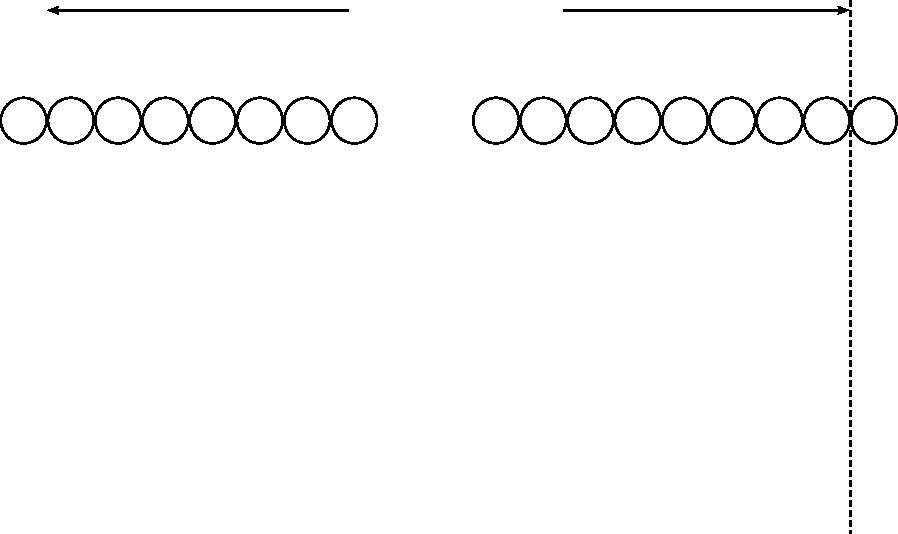
\includegraphics[width=1\linewidth]{./Diagrams/Process1}
\caption{Sensing processes with different types of objects. With a very slight object, there is Past Life-continuum and Vibrating Life-continuum but no Arresting Life-continuum and no Adverting.}
\label{fig:Process1}
\end{figure}

We now consider the different types of Sensing Processes. The Sensing Process shown in Handout 10 includes the Eye-consciousness Mind Moment. The Eye-door Process is the simple activity of seeing a small patch of colour. If we substitute Eye-consciousness with Ear-consciousness, we get the Ear-door Process, the simple activity of hearing a vibration. The Ear-door Process does not hear a song or a word, it hears only a vibration. Similarly, Eye-consciousness or Ear-consciousness can be replaced by Nose-consciousness, Tongue-consciousness or Body-consciousness resulting in simple activities at the other sense doors.

The Eye-door process shown in Handout 10 arises when there is a “very great object;” a \textbf{Visible-form} that immediately captures the attention of the mind. For a “very great object,” there is only one Past Life-continuum Mind Moment before the Vibrating Life-continuum arises. 

In the case of a “great object,” the mind’s attention is not immediately captured and two or three Past Life-continuum Mind Moments will arise before there is enough energy to stir the Vibrating Life-continuum Mind Moment. Since the duration of the Sensing Process is fixed,\footnote{The sense-object exists for the duration of 17 Mind Moments.} this means that for a “great object” there is time for seven Reaction Mind Moments but no time for Registration Mind Moments. Without Registration Mind Moments, there is no follow-up Thinking Process.

A “slight object” takes even more time to catch the mind’s attention. The “slight object” is processed with Five-sense-door Adverting, Sense-consciousness, Receiving, Investigating and Determining, but there is no time for Reaction Mind Moments to arise. A “very slight object” only vibrates the Life-continuum and does not even cause a Five-sense-door Adverting Mind Moment to arise.

\subsection*{Thinking Process}

\begin{figure}[h]
\centering
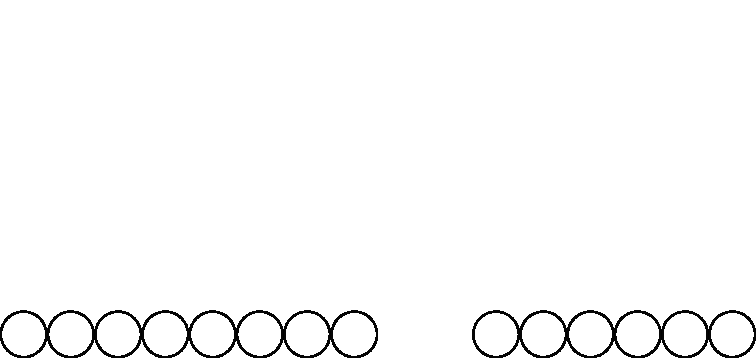
\includegraphics[width=0.8\linewidth]{./Diagrams/Process2}
\caption{An example of a Thinking Process; a Mind-door Process that shows how thinking happens without a thinker.}
\label{fig:Process2}
\end{figure}

So far, we have been analyzing the Sensing Process in some detail. This is useful as a model of how there can be seeing without a seer, but sensing has an almost insignificant effect on the kamma created. All of the weighty kamma created will come from the Thinking Process. The Thinking Process shows how there can be thinking without a thinker.

Using conventional language, we might say, “I see a car,” but according to the Abhidhamma, “seeing a car” involves far more thinking than seeing.

The eye-consciousness Mind Moment “sees” a small patch of colour. Once this small patch of colour (the Ultimate Reality) has been seen, it becomes a concept. Sensing is finished and now thinking takes over. The first thing that thinking does is the “grasp the object as a whole;” thinking builds up the entire field of vision from these “thumbnail-sized” patches of colour. How is this done? It is not in the linear way that a TV screen image is built up. Scientists say that the eye focuses first on areas of high contrast, on faces and on movement before filling in the rest of the scene.

Once the entire scene has been built up, the thinking mind recognizes colours. Next, a shape is extracted from the pattern of colours, the shape is recognized, a name is grasped (“car” in our example) and the name is recognized.\footnote{The process of converting an Ultimate Reality into a concept (\textit{tadanuvattikā manodvāravīthi}), grasping the object as a whole (\textit{samudāyagāhikā}), recognizing colours (\textit{vaṇṇasallakkhaṇā}), extracting a shape (\textit{vatthugāhikā}), recognizing the shape (\textit{vatthusallakkhaṇā}), grasping the name (\textit{nāmagāhikā}) and recognizing the name (\textit{nāmasallakkhaṇā}) were described by Ledi Sayādaw about 100 years ago.} Of course, next comes associations and judgements regarding the car, obsessions and fantasies about the car.

In summary, what we actually see is the Ultimate Reality of a small patch of colour. After seeing this small patch of colour, the Thinking Processes take over.

\subsubsection*{Types of Thinking Process}

The example of a Thinking Process shown in Handout 10 looks like a simplified version of the example of a Sensing Process. The difference between the two is that the Thinking Process does not have Five-sense-door Adverting, Sense-consciousness, Receiving or Investigating Mind Moments and jumps directly from Life-continuum to Determining\footnote{When Mind Moment \textbf{29} arises as part of a Thinking Process, it is called “Mind-door adverting consciousness; just as the five-sense-door adverting consciousness is the stage at which \textbf{Attention} is drawn towards a disturbance at the eye-door, the mind-door adverting consciousness is the stage at which \textbf{Attention} is drawn towards a disturbance at the mind-door. At this point, the direction of the mind is changing, turning around, adverting towards the mind-door.} and then Reacting. In other words, once the object is already in the mind, the Thinking Process jumps directly to determining and reacting, which generally leads to more determining and reacting with the same mental object as the mind spins out of control.

There are two types of Thinking Processes; a Thinking Process that ends with two Registration Mind Moments\footnote{Thinking Processes with a “clear object” (\textit{vibhūtālambana}) end with two Registration Mind Moments.} and a Thinking Process that ends with Reaction Mind Moments.\footnote{Thinking Processes with an “obscure object” (\textit{avibhūtālambana}) end with Reaction Mind Moments.} The Thinking Process that ends with two Registration Mind Moments marks the object so that the object can be picked up and further processed by subsequent Thinking Processes. The object of a Thinking Process that ends with Reaction Mind Moments will not be further processed by subsequent Thinking Processes.

\subsection*{Death and Rebirth Process}

\begin{figure}[h]
\centering
\input{./Diagrams/Death.pdf_tex}
\caption{Example of a death and rebirth process.}
\label{fig:Death}
\end{figure}

We now move on to the example of a Death and Rebirth Process shown at the bottom of Handout 10. 

Near the end of the old existence, there is a series of Reaction Mind Moments.\footnote{This is the “Death Process” and has five Reaction Mind Moments rather than seven Reaction Mind Moments. With only five Reaction Mind Moments, the kamma from the Death Process is not strong enough to generate productive kamma, it generates supportive kamma. In other words, the Death Process does not create the rebirth-linking kamma, but it supports the rebirth-linking kamma.} The object of these Reaction Mind Moments will be kamma, sign of kamma or sign of destiny from the old existence. This will become the object of the Life-continuum Mind Moments of the new existence. 

After the last Reaction Mind Moment, a single Life-continuum Mind Moment arises. This Life-continuum Mind Moment is the last Mind Moment in the old existence, so it is given the name “Death Mind Moment.” Just like all the previous Life-continuum Mind Moments from the old existence, the object of this Mind Moment is kamma, sign of kamma or sign of destiny from the prior existence, from the existence just before the old existence.

Immediately following the last Life-continuum Mind Moment from the old existence, the first Life-continuum Mind Moment from the new existence will arise. This first Life-continuum Mind Moment is new and different from the Life-continuum Mind Moments from the old existence. This first Life-continuum Mind Moment is called the Rebirth-linking Mind Moment and it takes as its object whatever was the object of the last Reaction Mind Moments from the old existence.

According to the Abhidhamma, the falling away of the “Death” Mind Moment in one existence is a condition for the immediate arising of the “Rebirth-linking” Mind Moment in the subsequent existence. In other words, Theravāda does not allow for any interim state between two lives. The lifespan of the new existence may be very short, even a matter of minutes, but it is considered to be a separate existence.

The first Life-continuum Mind Moment in the new existence is followed by 16 more identical Life-continuum Mind Moments and then the first Thinking Process of the new existence. The first thought of the new existence is the \textbf{Attachment} to the new existence.

\subsubsection*{Types of Death and Rebirth Process}

The Commentaries describe various types of Death and Rebirth Processes. Sometimes the Reaction Mind Moments from the old existence are from a Sensing Process, sometimes they are from a Thinking Process, sometimes the last process in the old existence ends with registration Mind Moments before the Death Mind Moment. These variations are technical details without any practical implications.

\subsection*{Arising and Cessation of \textit{Rūpa}}

We can also use the example of a Sensing Process and the example of a Death and Rebirth Process diagram to discuss the arising and cessation of \textit{rūpa}. As shown in Handout 5, groups of \textit{rūpas} can be temperature-born, kamma-born, mind-born and nutriment born.

Looking first at the example of a Sensing Process at the top of Handout 10, we can see that the lifespan of groups of \textit{rūpas} is the duration of 17 Mind Moments.\footnote{According to the Commentary, kamma-born groups and temperature-born groups arise at each of these three sub-moments of the Mind Moment (arising, presence and dissolution sub-moments) while mind-born groups and nutriment-born groups only arise at the arising sub-moment.} According to the Commentary, all groups of \textit{rūpas} have the same lifespan.\footnote{The lifespan of the object of a Thinking Process is not fixed.}

Now let us look at the Death and Rebirth Process diagram at the bottom of Handout 10 and consider the cessation of each group of \textit{rūpas} in the old existence and the arising of each group of \textit{rūpas} in the new existence. 

\begin{figure}[h]
\centering
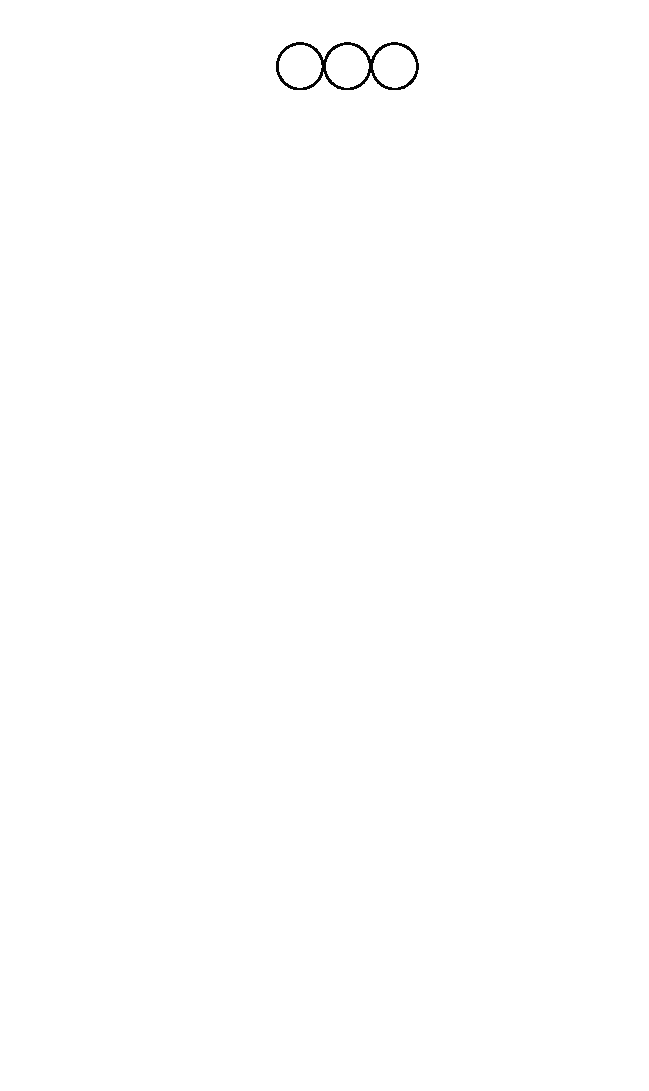
\includegraphics[width=0.5\linewidth]{./Diagrams/NewRupa}
\caption{Groups of rūpas during the first three Mind Moments of a new existence. Three new kamma-born groups are formed in every sub-moment (vital-nonad, gender, Heart-base). One new mind-born group is formed in every Mind Moment. For every new group formed in the previous sub-moment, a new temperature-born group is formed.}
\label{fig:NewRupa}
\end{figure}

Kamma-born groups of \textit{rūpas} are the living parts of the body. The last kamma-born group of \textit{rūpas} originates 17 Mind Moments before Death, so that when the Death Mind Moment falls away, there are no more kamma-born groups of \textit{rūpas} in the old existence. Three kamma-born groups of \textit{rūpas} arise together with the Rebirth-linking Mind Moment in the new existence: the vital-nonad group which gives life to the new existence, the Heart-base group which supports the Mind Moments of the new existence and the gender group, either femininity-group or masculinity group. The other kamma-born groups of \textit{rūpas}, the five sensitivities, will arise in the new existence when the respective sense organs have been formed. For example, the kamma-born group of \textit{rūpas} that is \textbf{Eye-sensitivity} will form once the physical eye has been formed.

Mind-born groups of \textit{rūpas} are created by Mind Moments. Every Mind Moment of the old existence, including the Death Mind Moment, will create mind-born groups of \textit{rūpas}, but after the Death Mind Moment, there will be no more mind-born groups of \textit{rūpas} created in the old existence. The first mind-born group of \textit{rūpas} in the new existence will arise during the Life-continuum Mind Moment immediately following the Rebirth-linking Mind Moment.

Temperature-born groups of \textit{rūpas} are the non-living parts of the body. After death, the temperature-born groups of \textit{rūpas} will continue to exist as the corpse. In the Rebirth-process, the first temperature-born groups of \textit{rūpas} of the new existence will arise during the Rebirth-linking Mind Moment.\footnote{During the arising sub-moment of the Rebirth-linking Mind Moment, there are only three kamma-born groups of \textit{rūpas}; the first temperature-born groups of \textit{rūpas} arise during the presence sub-moment of the Rebirth-linking Mind Moment.}

Nutriment-born groups of \textit{rūpas} depend on nutriment that has been taken in by the body. According to the Commentary, nutriment taken in by the body can create nutriment-born groups of \textit{rūpas} for up to seven days after being ingested. Therefore, the last nutriment-born groups of \textit{rūpas} in the old existence will fall away within seven days of death. The first nutriment-born groups of \textit{rūpas} in the new existence arise when the mother’s blood starts delivering nutriment to the new being.

\subsection*{Summary of Key Points}

Here is a summary of key points regarding Processes:

\begin{itemize}

\item Processes are models for “seeing without a seer” and “thinking without a thinker”.

\item Guarding the senses is an extremely important aspect of spiritual development:

\begin{itemize}

\item “Where would I possibly find enough leather with which to cover the surface of the earth? But just leather on the soles of my shoes is equivalent to covering the earth with it. Likewise, it is not possible for me to restrain the external course of things, but should I restrain my own mind, what would be the need to restrain all else?”

\end{itemize}

\item Ball of Honey Sutta: language for sensing is objective (describing an impersonal law of nature), language for thinking is subjective (describing an individual’s reaction).

\item Sensing takes Ultimate Realities as object, whereas thinking deals with names, ideas, concepts, judgements, obsessions and fantasies.

\item The Suttas define four of the five aggregates (all except rūpa) using terms related to sensing and thinking.

\item Key sections of dependent origination can also be viewed from a perspective of sensing and thinking.

\item A man sleeps beneath a mango tree (Stream of Life-continuum). A wind strikes the tree (Past Life-continuum). The branches sway with the wind (Vibrating Life-continuum). A mango falls beside the sleeping man (Arresting Life-continuum). The man awakes (Five-sense-door Adverting). The man opens his eyes (Eye-consciousness). The man picks up the mango (Receiving). The man presses and smells the mango (Investigating). The man understands that this is a mango fruit that is ripe and ready to eat (Determining). The man eats the mango (Reaction). The man notes the after-taste; his saliva still retains the mango taste (Registration). The man falls back to sleep (Stream of Life-continuum).

\item Kamma created by the sensing process is insignificant as compared to the kamma created by the subsequent thinking processes.

\begin{itemize}

\item Sensing process “sees” a small patch of colour; subsequent thinking processes build the field of vision, recognize things (“car”) and mentally proliferate.

\end{itemize}

\item Death and rebirth are also natural processes (with no gap in between).

\end{itemize}

Finally, in my opinion, the most important thing to remember about processes is that they are simple models of natural progressions. In my opinion, the technical details are not very important; what is important is the acceptance that sensing, thinking and rebirth are natural processes that do not need a Self to direct them.

Okay, we have come to the end of the course. I hope that you found this course to be interesting, practical and inspiring.

\begin{center}
\textbf{\textit{Sādhu! Sādhu! Sādhu!}} \\
\end{center}

\newpage

\subsection*{Questions \& Answers}

\question{What is the difference between death and parinibbāna?}

The word “\textit{Nibbāna}” literally means “extinguishing.” When one experiences \textit{Nibbāna} it can have the effect\footnote{Sotāpanna path Mind Moment extinguishes the fetters of personality-belief, \textbf{Doubt} and clinging to rites and rituals. Anāgāmī path Mind Moment extinguishes the fetters of sensuous craving and ill will. Arahat path Mind Moment extinguishes the five higher fetters of craving for fine-material existence, craving for immaterial existence, \textbf{Conceit}, \textbf{Restlessness} and \textbf{Delusion}.} of “extinguishing” the fetters that bind one to saṃsāra.

The Pāḷi prefix “pari” means “completely,” so \textit{parinibbāna} means the complete extinction of not only the fetters, but also the extinction of the five aggregates. A monk was scolded\footnote{SN 22.85: \url{ http://www.accesstoinsight.org/tipitaka/sn/sn22/sn22.085.than.html}} for having the \textbf{Wrong view} of “an Arahat does not exist after death;” according to the Commentary, the correct view would be “at the time of death, the process of arising and falling away of aggregates stops.”

\question{The Buddha had a gradual seven-step path to train monks, with each step building on the previous steps. Does this mean one should acquire at least certain level of skill in the preliminary steps, i.e., morality, guarding the senses and moderation with food before attempting to \color{blue} practise\color{black} meditation or attend a meditation retreat?}

Morality, guarding the senses and moderation in eating is an integral part of a meditation retreat. If you “cheat” and do not take these \color{blue} practices\color{black} seriously during your meditation retreat, then your meditation will not progress smoothly (your mind will be disturbed). Practising morality, guarding the senses and moderation in eating is also good preparation to be undertaken before a meditation retreat to train the mind and body. 

\question{How to \color{blue} practise\color{black} “guarding the senses” during daily life?}

The unguarded mind tends to spin out of control at every opportunity. This is how the defilements continually nourish and reinforce themselves. One must guard the senses during daily life by building a habit of \textbf{Mindfulness}. The earlier talks stressed the importance of using the \textbf{\textit{RADICAL}} technique, using your knowledge of the Abhidhamma to help \textbf{\textit{R}}ecognize and build a habit of \textbf{Mindfulness} during daily life.

The mind will have already started spinning out of control when you \textbf{\textit{R}}ecognize what is happening in the present moment. That is okay. With increased \color{blue} practice\color{black}, the mind will naturally start to \textbf{\textit{R}}ecognize what is happening at an earlier stage. Some meditation teachers have recommended putting aside one minute each hour to focus on \textbf{Mindfulness}. 

One of the training rules for monks and nuns is to keep their eyes lowered, to about five feet in front of them. The purpose of this rule is decorum,\footnote{Other rules in the same category of training rules include not laughing loudly and not swinging the arms.} but some meditation teachers recommend that yogis follow this \color{blue} practice\color{black} (when not on the cushion) to limit distractions. Personally, I find this to be very effective.
